\section{Experiments \& Deploment}\label{sec:experiments}

\subsection{Setup}

Simulations were run on 49 virtual machines in google cloud all co-located in
the same data center. The configuration of the nodes used was 4 CPU cores, 4
gigabytes of RAM, with a 10 gigabyte SSD running Ubuntu 22.4. The honest party
had an artificial network delay beetween 100-1000ms. This delay was achieved by
adding a sleep on every block message broadcast. Adversaries network delay was
only the inherent delay in communication between virtual machines and was <5 ms.
The tests were coordinated using ansible and the machines were given 2 minutes
to peer and stabalize at the beginning of each test. Thirty-seven nodes were
honest particpents and 12 nodes were configured as advisersaries.
Per\cite{eiar} it has been shown the most effective adversarial attack is a
private mining attack, which the adversarial nodes conducted during this
investigation. This configuration establishes the adversary's hash rate, denoted
to $\beta=0.244$ for our experiments. Both Bitcoin and PoEM were run on the same codebase
with the exception of modification to the consensus rule. Our primary objective is to
measure the confirmation delay (denoted as $d$) under varying block rates ($g$)
for both PoEM and Bitcoin protocols.

For each experimental setup, we fixed the value of $g$ and conducted a Monte
Carlo simulation comprising 100 iterations. In each iteration, we determined
the winner of each round by identifying which party reached that round quickest
from the experiment's onset. Upon completing 100 iterations, we aggregated the
victories of the honest party for each run. We then calculated the block
height, $K^*$, for which the probability of the honest parties' victory
surpasses 90\%. The chain growth rate, $f$, was found by taking the lifetime of
the execution and dividing the longest honest chain length with that lifetime.
The confirmation delay ($d$) for each experiment was obtained by dividing
$K^*$by $f$.

Figure 1 illustrates the evolution of $d$ across different $g$ values. We
identified the best operating conditions for a protocol as the point where the
confirmation delay is minimized. In our simulations, Bitcoin achieved its lowest
delay of 25.58$\Delta$ at a block rate of $g=0.98$. Conversely, PoEM for the
same blockrate reached its minimal delay of 18.29$\Delta$ with a
$\gamma=10$.This means for Bitcoin's best operating condition, the confimation
delay was 39.9\% higher compared to PoEM for the same block production rate.

Further, we extended our simulation to examine PoEM's performance with varied
bias values, specifically at Bitcoin's optimal operating point of $g=0.98$.
Figure 2 presents the confirmation delays corresponding to different bias
values. These results demonstrate that PoEM can achieve even lower confirmation
delays with optimized $\gamma$ values. Notably, the optimal confirmation delay
of 18.29 was observed at a bias setting of 10. However, the optimization of
$\gamma$ for all values of $g$ is a non-trivial task, and we leave this to
future work.

In addition to enhancing the confirmation delay, our study reveals that PoEM
also significantly improves the rate of chain growth, denoted as $f$.
Specifically, PoEM increases $f$ from 0.43 to 0.5, marking a 16.3\%
improvement, for a comparable confirmation delay (Bitcoin($d=25.6$),
PoEM($d=27.4$))

The increased chain growth rate is directly correlated with a higher realized
throughput for a blockchain system. Thus, PoEM not only demonstrates a
reduction in confirmation delay but also facilitates a higher transaction
throughput. This dual advantage positions PoEM as a notably efficient
blockchain protocol, offering substantial improvements over existing systems
like Bitcoin in terms of both processing speed and transactional capacity.

\begin{figure}
    \centering
    \begin{subfigure}{0.49\textwidth}
    \centering
    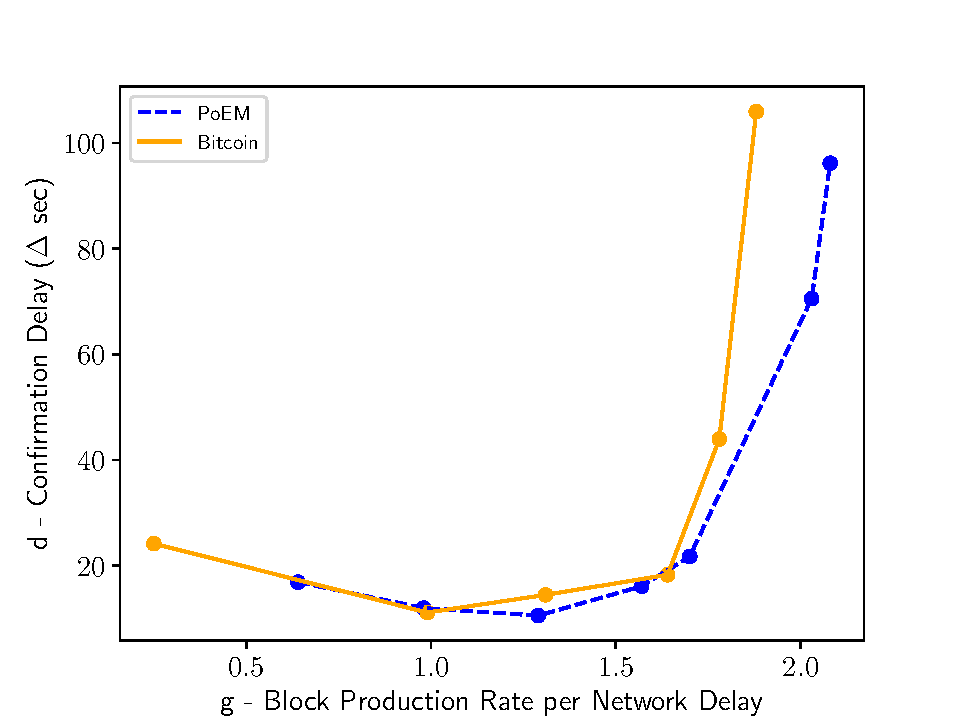
\includegraphics[width = 0.8\textwidth]{figures/dvsg.pdf}
    \caption{d vs g}
    \label{fig:dvsg}
    \end{subfigure}
    \begin{subfigure}{0.49\textwidth}
    \centering
    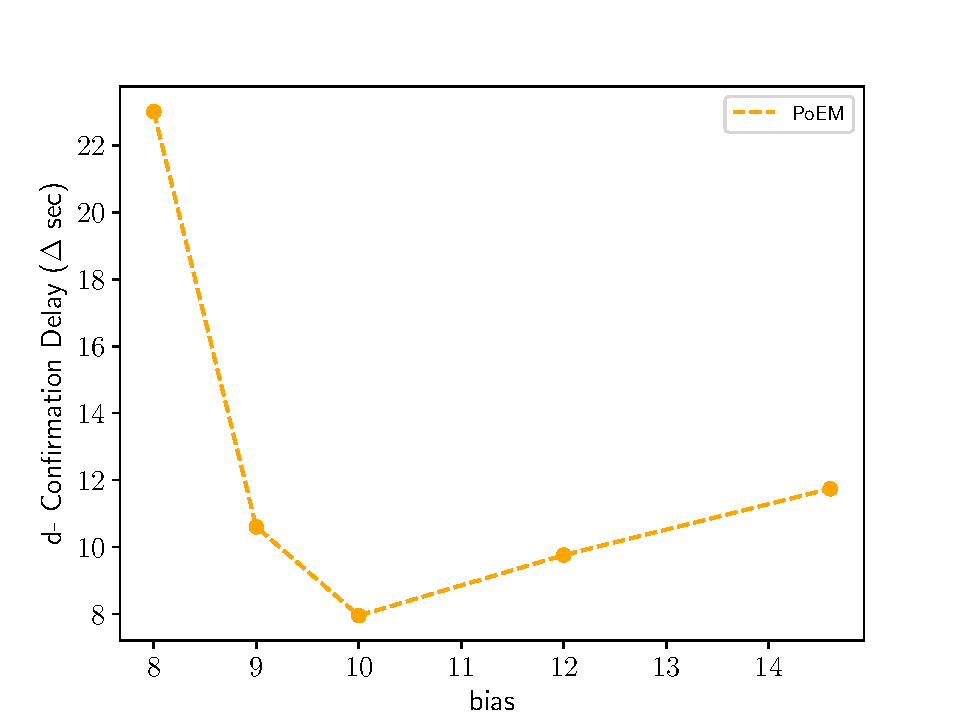
\includegraphics[width = 0.8\textwidth]{figures/gamma.pdf}
    \caption{d vs bias}
    \label{fig:bias}
    \end{subfigure}
    \begin{subfigure}{0.49\textwidth}
    \centering
    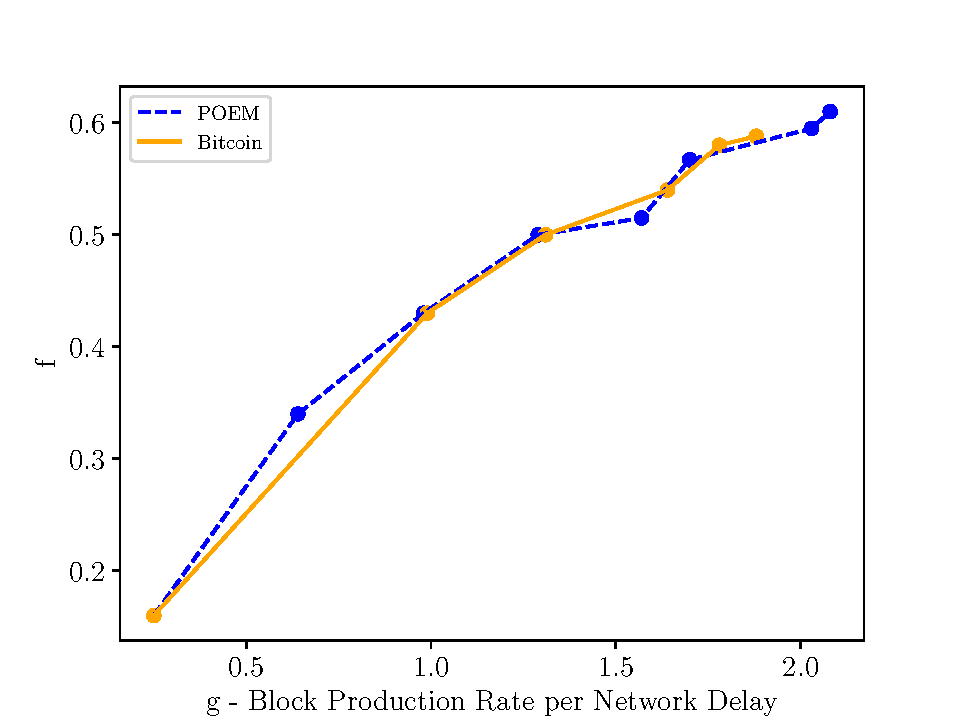
\includegraphics[width = 0.8\textwidth]{figures/fvg.pdf}
    \caption{f vs g}
    \label{fig:fg}
    \end{subfigure}
    \caption{Confirmation delay from simulations of PoEM and Bitcoin for various values of $g$ a) Confirmation delay $\Delta$ vs. the block production rate $g$. Note that PoEM typically demonstrates lower confirmation delay for any given value of $g$, and the difference becomes more pronounced at large $g$ b) Confirmation delay ($\Delta$) vs. the bias $\gamma$. The bias, $\gamma$ was experimentally optimized for the $g$ which showed the lowest confirmation delay in Bitcoin to elucidate the optimized performance of PoEM. PoEM achieved confirmation 39.9\% faster than Bitcoin's most optimal performance.}
    \label{fig:gamma}
\end{figure}

\subsection{Real-world Deployment}
In addition to
its success in simulations, PoEM has been effectively tested in a real-world,
permissionless peer-to-peer setting. During this
period, the network generated over 7.5 million blocks with participation from
more than 2000 miners/node operators. Moreover, PoEM has facilitated the
confirmation of over 500 million transactions. This deployment maintained an
average hash rate exceeding 50GH/s using the ProgPoW hash algorithm. Over the
network operation more than 51 petahashes total hash queries have been performed.
Network ran in variable difficulty setting with difficulty varying between 18
and 790 billion and $\gamma$ varying between 32 and 38.

Remarkably, even at sustained and high orphan rates upto 38\% PoEM maintained
finalization guarantees with practical confirmation delays. This has not been
achieved by a real world permissionless, work-based consensus blockchains under
such conditions. This real-world performance not only validates PoEM's efficacy
but also highlights its potential as a robust and scalable blockchain consensus
mechanism.
